\documentclass[tikz,border=10pt]{standalone}
\usepackage{tikz}
\usetikzlibrary{shapes.geometric, arrows.meta, positioning, calc, fit, backgrounds}
\usepackage{amsmath,amssymb}
\usepackage{xcolor}

% Unified Academic Color Palette
\definecolor{cInput}{RGB}{235, 248, 255}
\definecolor{bInput}{RGB}{49, 130, 206}

\definecolor{cTrans}{RGB}{240, 249, 255}
\definecolor{bTrans}{RGB}{43, 108, 176}

\definecolor{cGCN}{RGB}{230, 255, 250}
\definecolor{bGCN}{RGB}{49, 151, 149}

\definecolor{cRecurr}{RGB}{250, 245, 255}
\definecolor{bRecurr}{RGB}{128, 90, 213}

\definecolor{cHead}{RGB}{255, 245, 245}
\definecolor{bHead}{RGB}{229, 62, 62}

\definecolor{cFusion}{RGB}{254, 252, 191}
\definecolor{bFusion}{RGB}{214, 158, 46}

\definecolor{cGray}{RGB}{247, 250, 252}
\definecolor{bGray}{RGB}{160, 174, 192}

\definecolor{tDark}{RGB}{26, 32, 44}
\definecolor{tMuted}{RGB}{74, 85, 104}

\begin{document}
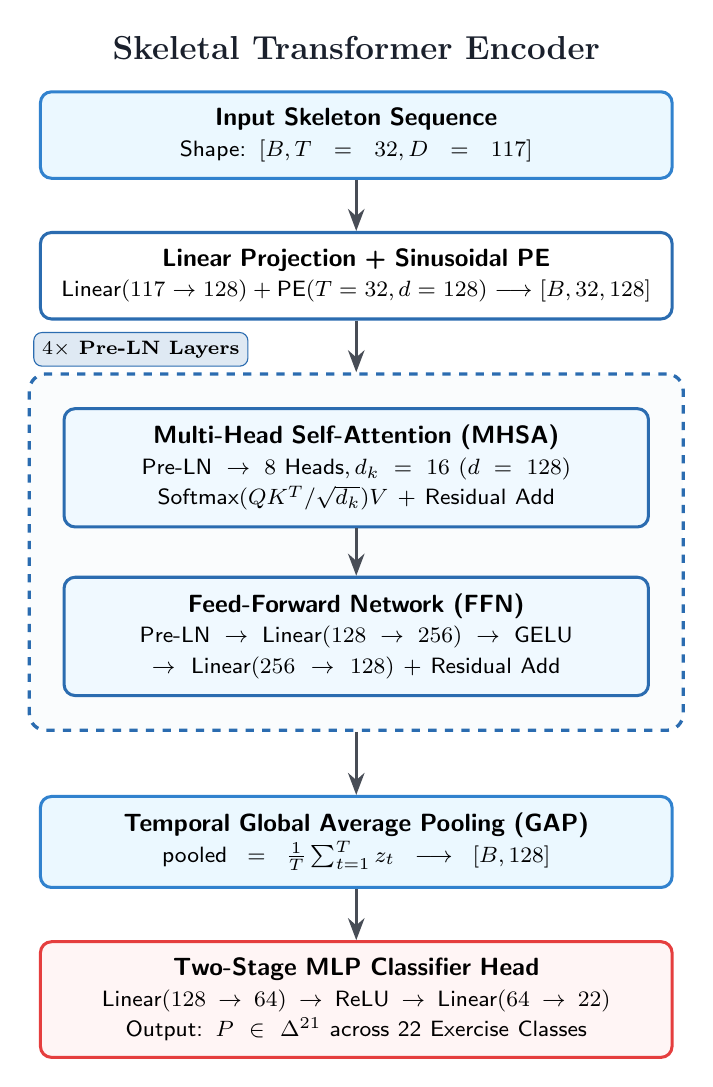
\begin{tikzpicture}[
    font=\sffamily\small,
    >=Stealth,
    node distance=0.65cm,
    block/.style={
        draw=#1,
        line width=1.1pt,
        rounded corners=4pt,
        align=center,
        inner sep=6pt
    },
    arrow/.style={->, line width=1.1pt, color=tDark!80}
]

\node[font=\bfseries\large, text=tDark] (title) at (0, 1.1) {Skeletal Transformer Encoder};

\node[block=bInput, fill=cInput, text width=7.6cm] (input) at (0, 0) {
    \textbf{Input Skeleton Sequence}\\
    {\footnotesize Shape: $[B, T=32, D=117]$}
};

\node[block=bTrans, fill=white, text width=7.6cm, below=of input] (proj) {
    \textbf{Linear Projection + Sinusoidal PE}\\
    {\footnotesize $\text{Linear}(117 \to 128) + \text{PE}(T=32, d=128) \longrightarrow [B, 32, 128]$}
};

% Container for 4x Encoder layers
\node[block=bTrans, fill=cTrans, text width=7.0cm, below=1.1cm of proj] (mhsa) {
    \textbf{Multi-Head Self-Attention (MHSA)}\\
    {\footnotesize $\text{Pre-LN} \to 8 \text{ Heads}, d_k=16 \ (d=128)$}\\
    {\footnotesize $\text{Softmax}(QK^T / \sqrt{d_k})V + \text{Residual Add}$}
};

\node[block=bTrans, fill=cTrans, text width=7.0cm, below=0.6cm of mhsa] (ffn) {
    \textbf{Feed-Forward Network (FFN)}\\
    {\footnotesize $\text{Pre-LN} \to \text{Linear}(128 \to 256) \to \text{GELU}$}\\
    {\footnotesize $\to \text{Linear}(256 \to 128) + \text{Residual Add}$}
};

\begin{scope}[on background layer]
    \node[draw=bTrans, line width=1.2pt, dashed, rounded corners=6pt, fill=cGray!60,
          fit=(mhsa)(ffn), inner sep=12pt] (cont) {};
    \node[anchor=south west, font=\bfseries\scriptsize, fill=bTrans!15, draw=bTrans, rounded corners=3pt, inner sep=3pt, xshift=2pt, yshift=2pt] at (cont.north west) {
        $4\times$ Pre-LN Layers
    };
\end{scope}

\node[block=bInput, fill=cInput, text width=7.6cm, below=0.8cm of cont] (gap) {
    \textbf{Temporal Global Average Pooling (GAP)}\\
    {\footnotesize $\text{pooled} = \frac{1}{T}\sum_{t=1}^T z_t \longrightarrow [B, 128]$}
};

\node[block=bHead, fill=cHead, text width=7.6cm, below=of gap] (head) {
    \textbf{Two-Stage MLP Classifier Head}\\
    {\footnotesize $\text{Linear}(128 \to 64) \to \text{ReLU} \to \text{Linear}(64 \to 22)$}\\
    {\footnotesize Output: $P \in \Delta^{21}$ across 22 Exercise Classes}
};

\draw[arrow] (input) -- (proj);
\draw[arrow] (proj) -- (cont);
\draw[arrow] (cont) -- (gap);
\draw[arrow] (gap) -- (head);
\draw[arrow] (mhsa) -- (ffn);

\end{tikzpicture}
\end{document}
